%%%%(c)
%%%%(c)  This file is a portion of the source for the textbook
%%%%(c)
%%%%(c)    Abstract Algebra: Theory and Applications
%%%%(c)    Copyright 1997 by Thomas W. Judson
%%%%(c)
%%%%(c)  See the file COPYING.txt for copying conditions
%%%%(c)
%%%%(c)
\chap{Lattices and Boolean Algebras}{boolean}

The axioms of a ring give structure to the operations of addition and multiplication on a set.  However, we can construct algebraic structures, known as lattices and Boolean algebras, that generalize other types of operations.  For example, the important operations on sets are inclusion, union, and intersection.  Lattices  are generalizations of order relations on algebraic spaces, such as set inclusion in set theory and inequality in the  familiar number systems ${\mathbb N}$, ${\mathbb Z}$, ${\mathbb Q}$, and ${\mathbb R}$.  Boolean algebras generalize the operations of intersection and union. Lattices and Boolean algebras have found applications in logic, circuit theory, and probability.   


\section{Lattices}\label{boolean_lattices}

\subsection*{Partially Ordered Sets}

We begin by the study of lattices and Boolean algebras by generalizing the idea of inequality. Recall that a \boldemph{relation} on a set $X$ is a subset of $X \times X$.  A relation $P$ on $X$ is called a \boldemph{partial order}\index{Partial order} of $X$ if it satisfies the following axioms.  
\begin{enumerate}

\item
The relation is \boldemph{reflexive}: $(a, a) \in P$ for all $a \in X$.

\item
The relation is \boldemph{antisymmetric}: if $(a,b) \in P$ and $(b,a) \in P$, then $a = b$.

\item
The relation is \boldemph{transitive}: if $(a, b) \in P$ and $(b, c) \in P$, then $(a, c) \in P$.
 
\end{enumerate}
We will usually write $a \preceq b$\label{lessthan} to mean $(a, b) \in P$  unless some symbol is naturally associated with a particular partial order, such as $a \leq b$ with integers $a$ and $b$, or $X \subseteq Y$ with sets $X$ and $Y$.  A set $X$ together with a partial order $\preceq$ is called a \boldemph{partially ordered set},\index{Partially ordered set} or \boldemph{poset}\index{Poset!definition of}. 

\begin{example}{Z_less_equal}
The set of integers (or rationals  or reals) is a poset where $a \leq  b$ has the usual meaning for two integers $a$ and $b$ in ${\mathbb Z}$.
\end{example}


\begin{example}{power_set_subset}
Let $X$ be any set.  We will define the \boldemph{power set\/}\index{Power set} of $X$ to be the set of all subsets of $X$. We denote the power set of $X$ by ${\mathcal P}(X)$. For example, let $X = \{ a, b, c \}$.  Then ${\mathcal P}(X)$ is  the set of all subsets of the set  $\{ a, b, c \}$: 
\[
\begin{array}{cccc}
\emptyset & \{ a \} & \{ b \} & \{ c \} \\
\{ a, b \} & \{ a, c\} &\{ b, c\} & \{ a, b, c \}.
\end{array}
\]
On any power set of a set $X$, set inclusion, $\subseteq$, is a partial order.  We can represent the order on $\{ a, b, c \}$ schematically by a diagram such as the one in  Figure~\ref{partial}. 
\end{example}

\begin{figure}[htb]
\begin{center}
\tikzpreface{boolean_order_abc}
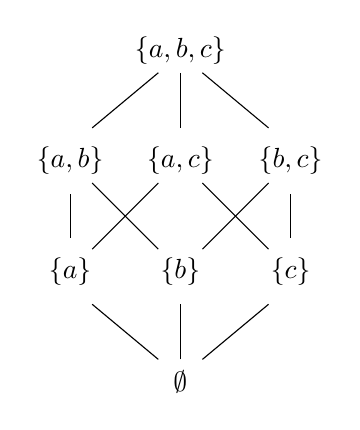
\begin{tikzpicture}[scale=0.7] %Replaced figure with tikz figure and corrected figure - TWJ 8/17/2010

\draw  (0,2.6) -- (0,1.6);
\draw  (0,-2.6) -- (0,-1.6);

\draw  (2,0.4) -- (2,-0.4);
\draw  (-2,0.4) -- (-2,-0.4);

\draw  (1.6,1.6) -- (0.4,2.6);
\draw  (-1.6,-1.6) -- (-0.4,-2.6);
\draw  (-1.6,1.6) -- (-0.4,2.6);
\draw  (1.6,-1.6) -- (0.4,-2.6);

\draw  (1.6,0.6) -- (0.4,-0.6);
\draw  (-1.6,0.6) -- (-0.4,-0.6);

\draw  (0.4,0.6) -- (1.6,-0.6);
\draw  (-0.4,0.6) -- (-1.6,-0.6);

\node at (0, 3) {$\{ a, b, c \}$};
\node at (-2, 1) {$\{ a, b \}$};
\node at (0, 1) {$\{ a, c \}$};
\node at (2, 1) {$\{ b, c \}$};
\node at (-2, -1) {$\{ a \}$};
\node at (0, -1) {$\{ b \}$};
\node at (2, -1) {$\{ c \}$};
\node at (0, -3) {$\emptyset$};

\end{tikzpicture}
\end{center}
\caption{Partial order on ${\mathcal P}( \{ a, b, c \})$}
\label{partial}
\end{figure}

\begin{example}{subgroup_poset}
Let $G$ be a group. The set of subgroups of $G$ is a poset, where the partial order is set inclusion.
\end{example}


\begin{example}{poorder_not_unique}
There can be more than one partial order on a particular set.  We can form a partial order on ${\mathbb N}$ by $a \preceq b$ if $a \mid b$.  The relation is certainly reflexive since $a \mid a$ for all $a \in {\mathbb N}$.  If $m \mid n$ and $n \mid m$, then $m = n$; hence, the relation is also antisymmetric.  The relation is transitive, because if $m \mid n$ and $n \mid p$, then $m \mid p$.
\end{example}


\begin{example}{poset_div}
Let $X = \{ 1, 2, 3, 4, 6, 8, 12, 24 \}$ be the set of divisors of 24 with the partial order defined in Example~\ref{example:boolean:poorder_not_unique}. Figure~\ref{Poset1} shows the partial order on $X$. 
\end{example}


\begin{figure}[htb]
\begin{center}
\tikzpreface{boolean_order_24}
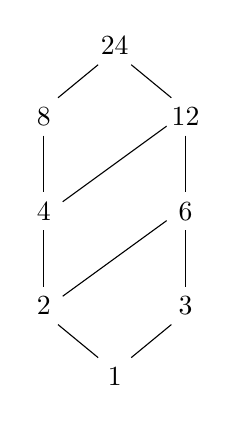
\begin{tikzpicture}[scale=0.6] %Replaced figure with tikz figure - TWJ 8/17/2010


\draw  (1.2,2.4) -- (0.35,3.1);
\draw  (-1.2,2.4) -- (-0.35,3.1);
\draw  (1.2,-2.4) -- (0.35,-3.1);
\draw  (-1.2,-2.4) -- (-0.35,-3.1);

\draw (1.5,1.6) -- (1.5,0.4);
\draw (-1.5,1.6) -- (-1.5,0.4);
\draw (1.5,-1.6) -- (1.5,-0.4);
\draw (-1.5,-1.6) -- (-1.5,-0.4);

\draw (-1.1,0.2) -- (1.1,1.8);
\draw (-1.1,-1.8) -- (1.1,-0.2);

\node at (0, 3.5) {24};

\node at (1.5, 2) {12};
\node at (1.5, 0) {6};
\node at (1.5, -2) {3};

\node at (-1.5, 2) {8};
\node at (-1.5, 0) {4};
\node at (-1.5, -2) {2};

\node at (0, -3.5) {1};

\end{tikzpicture}

\end{center}
\caption{A partial order on the divisors of 24}
\label{Poset1}
\end{figure}

Let $Y$ be a subset of a poset $X$. An element $u$ in $X$ is an \boldemph{upper bound}\index{Upper bound} of $Y$ if $a \preceq u$ for every element $a \in Y$. If $u$ is an upper bound of $Y$ such that $u \preceq v$ for every other upper bound $v$ of $Y$, then $u$ is called a \boldemph{least upper bound}\index{Least upper bound} or \boldemph{supremum}\index{Supremum} of $Y$. An element $l$ in $X$ is said to be a \boldemph{lower bound}\index{Lower bound} of $Y$ if $l \preceq a$ for all $a \in Y$. If $l$ is a lower bound of $Y$ such that $k \preceq l$ for every other lower bound $k$ of $Y$, then $l$ is called a \boldemph{greatest lower bound}\index{Greatest lower bound} or \boldemph{infimum}\index{Infimum} of $Y$.


\begin{example}{poset_gcd}
Let $Y = \{  2, 3, 4, 6 \}$ be contained in the set $X$ of Example~\ref{example:boolean:poset_div}.  Then $Y$ has upper bounds 12 and 24, with 12 as a least upper bound.  The only lower bound is 1; hence, it must be a greatest lower bound.
\end{example}


As it turns out, least upper bounds and greatest lower bounds are unique if they exist.

\begin{theorem}
Let $Y$ be a nonempty subset of a poset $X$. If $Y$ has a least upper bound, then $Y$ has a unique least upper bound. If $Y$ has a greatest lower bound, then $Y$ has a unique greatest lower bound.
\end{theorem} 

\begin{proof}
Let $u_1$ and $u_2$ be least upper bounds for $Y$. By the definition
of the least upper bound, $u_1 \preceq u$ for all upper bounds $u$ of
$Y$. In particular, $u_1 \preceq u_2$. Similarly, $u_2 \preceq u_1$.
Therefore, $u_1 = u_2$ by antisymmetry.  A similar argument show that
the greatest lower bound is unique.
\end{proof}
 
\medskip
 
On many posets it is possible to define binary operations
by using the greatest lower bound and the least upper bound of two
elements. A \boldemph{lattice}\index{Lattice!definition of} is a poset $L$
such that every pair of elements in $L$ has a least upper bound and a
greatest lower bound. The least upper bound of $a, b \in L$ is called
the \boldemph{join}\index{Join}\label{join} of $a$ and $b$ and is denoted 
by $a \vee b$.  The greatest lower bound of $a, b \in L$ is called 
the \boldemph{meet}\index{Meet}\label{meet} of $a$ and $b$ and is denoted 
by $a \wedge b$.
 
 

\begin{example}{lub_glb}
Let $X$ be a set. Then the power set of $X$, ${\mathcal P}(X)$, is a
lattice. For two sets $A$ and $B$ in ${\mathcal P}(X)$, the least upper
bound of $A$ and $B$ is $A \cup B$. Certainly $A \cup B$ is an upper
bound of $A$ and $B$, since $A \subseteq A \cup B$ and $B \subseteq A
\cup B$.  If $C$ is some other set containing both $A$ and $B$, then
$C$ must contain $A \cup B$; hence, $A \cup B$ is the least upper bound
of $A$ and $B$. Similarly,  the greatest lower bound of $A$ and $B$ is
$A \cap B$.
\end{example}
 
 

\begin{example}{subgroup_lattice}
Let $G$ be a group and suppose that $X$ is the set of subgroups of
$G$.  Then $X$ is a poset ordered by set-theoretic inclusion,
$\subseteq$.  The set of subgroups of $G$ is also a lattice.  If $H$
and $K$ are subgroups of $G$, the greatest lower bound of $H$ and $K$
is $H \cap K$. The set $H \cup K$ may not be a subgroup of $G$.  We
leave it as an exercise to show that the least upper bound of $H$ and
$K$ is the subgroup generated by $H \cup K$. 
\end{example}
 

 
 
In set theory we have certain duality conditions. For example, by De
Morgan's laws, any statement about sets that is true about $(A \cup
B)'$ must also be true about $A' \cap B'$. We also have a duality
principle for lattices. 
 
 
\medskip
 
 
\noindent \textbf{Principle of Duality.}\index{Lattices, Principle of
Duality for}
Any statement that is true for all lattices remains true when
$\preceq$ is replaced by $\succeq$ and $\vee$ and $\wedge$ are
interchanged throughout the statement.
 
 
\medskip
 
 
The following theorem tells us that a lattice is an algebraic
structure with two binary operations that satisfy certain
axioms.						     
 
 
\begin{theorem}
If $L$ is a lattice, then the binary operations $\vee$ and $\wedge$
satisfy the following properties for $a, b, c \in L$.
\begin{enumerate}
 
\rm \item \it
Commutative laws: $a \vee b = b \vee a$ and $a \wedge b = b \wedge a$.
 
\rm \item \it
Associative laws: $a \vee ( b \vee c) = (a \vee b) \vee c$ and $a \wedge (
b \wedge c) = (a \wedge b) \wedge c$. 
 
\rm \item \it
Idempotent laws: $a \vee a = a$ and $a \wedge a = a$.
 
\rm \item \it
Absorption laws: $a \vee (a \wedge b) = a$ and $a \wedge ( a \vee b ) =a$.
 
\end{enumerate}
\end{theorem}
 
 
\begin{proof}
By the Principle
of Duality, we need only prove the first statement in each part. 
 
 
(1)  
By definition $a \vee b$ is the least upper bound of $\{ a, b\}$, and
$b \vee a$ is the least upper bound of $\{ b, a \}$; however, $\{ a, b\} 
= \{ b, a \}$.
 
 
(2)
We will show that $a \vee ( b \vee c)$ and $(a \vee b) \vee c$
are both least upper bounds of $\{ a, b, c \}$.	 Let $d =  a \vee b$.
Then $c \preceq  d \vee c = (a \vee b) \vee c$. We also know that 
\[
a \preceq  a \vee b =d \preceq  d \vee c = (a \vee b) \vee c.
\]
A similar argument demonstrates that $b \preceq (a \vee b) \vee c$.
Therefore, $(a \vee b) \vee c$ is an upper bound of $\{ a, b, c \}$.
We now need to show that $(a \vee b) \vee c$ is the least upper bound
of $\{ a, b, c\}$. Let $u$ be some other upper bound of $\{ a, b, c \}$. 
Then $a \preceq u$ and $b \preceq u$; hence, $d = a \vee b \preceq u$.
Since $c \preceq u$, it follows that $(a \vee b) \vee c = d \vee c
\preceq u$. Therefore, $(a \vee b) \vee c$ must be the least upper 
bound of $\{ a, b, c\}$. The argument that shows  $a \vee ( b \vee c)$ 
is the least upper bound of $\{ a, b, c \}$ is the same.  Consequently,
$a \vee ( b \vee c) = (a \vee b) \vee c$.
 
 
(3)
The join of $a$ and $a$ is the least upper bound of $\{ a \}$; hence,
$a \vee a = a$.
 
 
(4)
Let $d = a \wedge b$. Then $a \preceq a \vee d$.  On the other hand,
$d = a \wedge b \preceq a$, and so $a \vee d \preceq a$.  Therefore,
$a \vee ( a \wedge b) = a$.
\end{proof}
 
 
\medskip
 
 
Given any arbitrary set $L$ with operations $\vee$ and $\wedge$, 
satisfying the conditions of the previous theorem, it is natural
to ask whether or not this set comes from some lattice.  The
following theorem says that this is always the case.
 
 
\begin{theorem}\label{boolean:PO_theorem}
Let $L$ be a nonempty set with two binary operations $\vee$ and
$\wedge$ satisfying the commutative, associative, idempotent, and  
absorption laws.  We can define a partial order on $L$ by  $a \preceq
b$ if $a \vee b = b$. Furthermore, $L$ is a lattice with respect 
to $\preceq$ if for all $a, b \in L$, we define the least upper bound
and greatest lower bound of $a$ and $b$ by $a \vee b$ and $a \wedge
b$, respectively.
\end{theorem}
 
 
\begin{proof}
We first show that $L$ is a poset under $\preceq$. Since $a \vee a =
a$, $a \preceq a$ and $\preceq$ is reflexive. To show that $\preceq$
is antisymmetric, let $a \preceq b$ and $b \preceq a$. Then $a \vee b
= b$ and $b \vee a = a$.  By the commutative law, $b = a \vee b
= b \vee a = a$.   Finally, we must show that $\preceq$ is
transitive. Let $a \preceq b$ and $b \preceq c$. Then $a \vee b = b$
and $b \vee c = c$.  Thus,
\[
a \vee c = a \vee (b \vee c ) = ( a \vee b) \vee c = b \vee c = c,
\]
or $a \preceq c$.
 
To show that $L$ is a lattice, we must prove that $a \vee b$ and $a
\wedge b$ are, respectively, the least upper and greatest lower bounds
of $a$ and $b$. Since $a=(a \vee b) \wedge a = a \wedge (a \vee b)$,
it follows that $a \preceq a \vee b$.  Similarly, $b \preceq a \vee
b$. Therefore, $a \vee b$ is an upper bound for $a$ and $b$. Let $u$
be any other upper bound of both $a$ and $b$. Then $a \preceq u$ and
$b \preceq u$. But $a \vee b \preceq u$ since 
\[
(a \vee b) \vee u = a \vee (b \vee u) = a \vee u = u.
\]
The proof that $a \wedge b$ is the greatest lower bound of $a$ and
$b$ is left as an exercise.
\end{proof}
 
 
 
\section{Boolean Algebras}
 
 
Let us investigate the example of the power set, ${\mathcal P}(X)$, of a
set $X$ more  closely. The power set is a lattice that is  ordered by
inclusion. By the definition of the power set, the largest element in
${\mathcal P}(X)$ is $X$ itself and the smallest element is $\emptyset$,
the empty set. For any set $A$ in ${\mathcal P}(X)$, we know that $A \cap
X = A$ and $A \cup \emptyset = A$. This suggests the following
definition for lattices. An element $I$\label{notelargeposet} 
in a poset $X$ is a \boldemph{
largest element}\index{Poset!largest element in} if $a \preceq I$ for
all $a \in X$.  An element $O$\label{notesmallposet} 
 is a  \boldemph{smallest
element}\index{Poset!smallest element in} of $X$ if $O \preceq a$ for
all $a \in X$.  
 
 
Let $A$ be in ${\mathcal P}(X)$. Recall that the complement of $A$ is
\[
A' = X \setminus A = \{ x : \mbox{ $x \in X$ and $x \notin A$}  \}.
\]
We know that $A \cup A' = X$ and $A \cap A' = \emptyset$. We can
generalize this example for lattices. A lattice $L$ with a largest
element $I$ and a smallest element $O$ is \boldemph{
complemented}\index{Lattice!completed} if for each $a \in X$, there
exists an $a'$\label{notedlatticecomp} 
such that $a \vee a' = I$ and $a \wedge a' = O$.
 
 
In a lattice $L$, the binary operations $\vee$ and $\wedge$ satisfy
commutative and associative laws; however, they need not satisfy the
distributive law 
\[ 
a \wedge ( b \vee c ) = (a \wedge b ) \vee ( a \wedge c );
\]
however, in ${\mathcal P}(X)$ the distributive law is satisfied since
\[
A \cap ( B \cup C ) = (A \cap B ) \cup ( A \cap C )
\]
for $A, B, C \in {\mathcal P}(X)$. We will say that a lattice $L$ is
\boldemph{distributive\/}\index{Lattice!distributive} if the following
distributive law holds:
\[
a \wedge ( b \vee c ) = (a \wedge b ) \vee ( a \wedge c )
\]
for all $a, b, c \in L$.
 
 
\begin{theorem}\label{boolean:dist_lattice_theorem}
A lattice $L$ is distributive if and only if 
\[
a \vee ( b \wedge c ) = ( a \vee b ) \wedge ( a \vee c )
\]
for all $a, b, c \in L$.
\end{theorem}
 
 
\begin{proof}
Let us assume that $L$ is a distributive lattice.
\begin{align*}
a \vee ( b \wedge c ) 
& = [a \vee (a \wedge c) ] \vee ( b \wedge c ) \\
& = a \vee [(a \wedge c)  \vee ( b \wedge c )] \\
& = a \vee [(c \wedge a)  \vee ( c \wedge b )] \\
& = a \vee [c \wedge ( a  \vee b )] \\
& = a \vee [( a  \vee b ) \wedge c ] \\
& = [( a  \vee b ) \wedge a ] \vee [(a \vee b) \wedge c ] \\
& = ( a \vee b ) \wedge ( a \vee c ).
\end{align*}
The converse follows directly from the Duality Principle.
\end{proof}
 
 
\medskip
 
 
A \boldemph{Boolean algebra}\index{Boolean algebra!definition of} is a
lattice $B$ with a greatest element $I$ and a smallest element $O$
such that $B$ is both distributive and complemented. The power set of
$X$, ${\mathcal P}(X)$, is our prototype for a Boolean algebra.  As it
turns out, it is also one of the most important Boolean algebras. The
following theorem allows us to characterize Boolean algebras in terms
of the binary relations $\vee$ and $\wedge$ without mention of the
fact that a Boolean algebra is a poset. 
 
 
\begin{theorem}
A set $B$ is a Boolean algebra if and only if there exist binary
operations $\vee$ and $\wedge$ on $B$ satisfying the following axioms.
\begin{enumerate}
 
\rm \item \it
$a \vee b = b \vee a$ and $a \wedge b = b \wedge a$ for $a, b \in B$.
 
\rm \item \it
$a \vee ( b \vee c) = (a \vee b) \vee c$ and 
$a \wedge ( b \wedge c) = (a \wedge b) \wedge c$ 
for $a, b, c \in B$.
 
\rm \item \it
$a \wedge ( b \vee c ) = (a \wedge b ) \vee ( a \wedge c )$ and 
$a \vee ( b \wedge c ) = (a \vee b ) \wedge ( a \vee c )$  
for $a, b, c \in B$.
 
\rm \item \it
There exist elements $I$ and $O$ such that $a \vee O = a$ and $a
\wedge I = a$ for all $a \in B$.
 
\rm \item \it
For every $a \in B$ there exists an $a' \in B$ such that $a \vee a' =
I$ and $a \wedge a' = O$.
 
\end{enumerate}
\end{theorem}
 
 
\begin{proof}
Let $B$ be a set satisfying (1)--(5) in the theorem.  One of the
idempotent laws is satisfied since
\begin{align*}
a & = a \vee O \\
& = a \vee (a \wedge a') \\
& = (a \vee a) \wedge (a \vee a') \\
& = (a \vee a ) \wedge I \\
& = a \vee a.
\end{align*}
Observe that 
\[
I \vee b = (I \vee b ) \wedge I = (I \wedge I) \vee (b \wedge I) = I
\vee I =  I.  
\]
Consequently, the first of the two absorption laws holds, since
\begin{align*}
a \vee (a \wedge b) & = (a \wedge I) \vee (a \wedge b) \\
& = a \wedge (I \vee b) \\
& = a  \wedge I \\
& = a.
\end{align*}
The other idempotent and absorption laws are proven similarly. Since
$B$ also satisfies (1)--(3), the conditions of Theorem~\ref{boolean:PO_theorem} are met;
therefore, $B$ must be a lattice.  Condition (4) tells us that $B$ is
a distributive lattice.
 
 
For $a \in B$, $O \vee a = a$; hence, $O \preceq a$ and $O$ is the
smallest element in $B$. To show that $I$ is the largest element in
$B$, we will first show that $a \vee b = b$ is equivalent to $a \wedge
b = a$.  Since $a \vee I = a$ for all $a \in B$, using the absorption
laws we can determine that
\[
a \vee I =(a \wedge I) \vee I = I \vee ( I \wedge a) = I
\]
or $a \preceq I$ for all $a$ in $B$. Finally, since we know that $B$
is complemented by (5), $B$ must be a Boolean algebra. 
 
 
Conversely, suppose that $B$ is a Boolean algebra. Let $I$ and $O$ be
the greatest and least elements in $B$, respectively.  If we define $a
\vee b$ and $a \wedge b$ as least upper and greatest lower bounds of
$\{ a, b\}$, then $B$ is a Boolean algebra by Theorem~\ref{boolean:PO_theorem} , 
Theorem~\ref{boolean:dist_lattice_theorem}, and our hypothesis. 
\end{proof}
 
 
\medskip
 
 
Many other identities hold in Boolean algebras.  Some of these
identities are listed in the following theorem. 
 
 
\begin{theorem}
Let $B$ be a Boolean algebra. Then
\begin{enumerate}
 
\rm \item \it
$a \vee I = I$ and $a \wedge O = O$ for all $a \in B$. 
 
\rm \item \it
If $a \vee b = a \vee c$ and $a \wedge b = a \wedge c$ for $a, b, c
\in B$, then $b = c$.
 
\rm \item \it
If $a \vee b = I$ and $a \wedge b = O$, then $b = a'$.
 
\rm \item \it
$(a')'=a$ for all $a \in B$.
 
\rm \item \it
$I' = O$ and $O' = I$.
 
\rm \item \it
$(a \vee b)' = a' \wedge b'$ and $(a \wedge b)' = a' \vee b'$ (De
Morgan's Laws)\index{De Morgan's laws!for Boolean algebras}.
 
\end{enumerate}
\end{theorem}
 
 
\begin{proof}
We will prove only (2). The rest of the identities are left as
exercises. For $a \vee b = a \vee c$ and $a \wedge b = a \wedge c$, we
have  
\begin{align*}
b & = b \vee (b \wedge a)  \\
& =  b \vee (a \wedge b)  \\
& =  b \vee (a \wedge c)  \\
& =  ( b \vee a) \wedge ( b \vee c)  \\
& =  ( a \vee b) \wedge ( b \vee c)  \\
& =  ( a \vee c) \wedge ( b \vee c)  \\
& =  ( c \vee a ) \wedge ( c\vee b )  \\
& = c \vee (a \wedge b) \\
& = c \vee ( a \wedge c ) \\
& = c \vee ( c \wedge a ) \\
& = c.
\end{align*}
\end{proof}
 
 
 
\subsection*{Finite Boolean Algebras}
 
 
A Boolean algebra is a \boldemph{finite Boolean algebra}\index{Boolean
algebra!finite} if it contains a finite number of elements as a set.
Finite Boolean algebras are particularly nice since we can classify
them  up to isomorphism.   
 
 
Let $B$ and $C$ be Boolean algebras.  A bijective map $\phi : B
\rightarrow C$ is an \boldemph{isomorphism}\index{Boolean
algebra!isomorphism}\index{Isomorphism!of Boolean algebras} of Boolean
algebras  if 
\begin{align*}
\phi( a \vee b )  & = \phi(a) \vee \phi(b) \\
\phi( a \wedge b )  & = \phi(a) \wedge \phi(b)
\end{align*}
for all $a$ and $b$ in $B$. 
 
 
% 2010/05/18 R Beezer, added a "nonzero" to  b  in definition of an atom
% Identified by Ricky Roy, U of Puget Sound
We will show that any finite Boolean algebra is isomorphic to the 
Boolean algebra obtained by taking the power set of some finite set 
$X$. We will need a few lemmas and definitions before we prove this result.
Let $B$ be a finite Boolean algebra. An element $a \in B$ is  an \boldemph{
atom}\index{Atom}\index{Boolean algebra!atom in a} of $B$ if $a \neq
O$ and $a \wedge b = a$ for all nonzero $b \in B$. Equivalently, $a$ is an
atom of $B$ if there is no nonzero $b \in B$ distinct from $a$ such
that $O \preceq b \preceq a$. 
 
 
\begin{lemma}
Let $B$ be a finite Boolean algebra. If $b$ is a nonzero element of
$B$, then there is an atom $a$ in $B$ such that $a \preceq b$.
\end{lemma}
 
 
\begin{proof}
If $b$ is an atom, let $a =b$. Otherwise, choose an element $b_1$, not
equal to $O$ or $b$, such that $b_1 \preceq b$. We are guaranteed that
this is possible since $b$ is not an atom. If $b_1$ is an atom, then
we are done.  If not, choose $b_2$, not equal to $O$ or $b_1$, such that 
$b_2 \preceq b_1$. Again, if $b_2$ is an atom, let $a = b_2$.
Continuing this process, we can obtain a chain
\[
O \preceq \cdots \preceq b_3 \preceq b_2 \preceq b_1 \preceq b.
\]
Since $B$ is a finite Boolean algebra, this chain must be finite.  That
is, for some $k$, $b_k$ is an atom. Let $a = b_k$.
\end{proof}
 
 
\begin{lemma}\label{boolean:zero_vee_lemma}
Let $a$ and $b$ be atoms in a finite Boolean algebra $B$ such that $a
\neq b$. Then $a \wedge b = O$.
\end{lemma}
 
 
\begin{proof}
Since $a \wedge b$ is the greatest lower bound of $a$ and $b$, we know
that $a \wedge b \preceq a$.  Hence, either $a \wedge b = a$ or $a
\wedge b = O$. However, if $a \wedge b = a$, then either $a \preceq b$
or $a = O$.  In either case we have a contradiction because $a$ and
$b$ are both atoms; therefore, $a \wedge b = O$. 
\end{proof}
 
 
\begin{lemma}\label{boolean:PO_equivalent_lemma}
Let $B$ be a Boolean algebra and $a, b \in B$. The following 
statements are equivalent. 
\begin{enumerate}
 
\rm \item \it
$a \preceq b$.
 
\rm \item \it
$a \wedge b' = O$.
 
\rm \item \it
$a' \vee b = I$.
 
\end{enumerate}
\end{lemma}
 
 
\begin{proof}
(1) $\Rightarrow$ (2).
If $a \preceq b$, then $a \vee b = b$. Therefore,
\begin{align*} 
a \wedge b' & = a \wedge (a \vee b)' \\
& = a \wedge ( a' \wedge b') \\
& = ( a \wedge a') \wedge b' \\     
& = O \wedge b' \\
& = O.
\end{align*}
 
 
(2) $\Rightarrow$ (3).
If $a \wedge b' = O$, then $a' \vee b = (a \wedge b')' = O' = I$. 
 
 
(3) $\Rightarrow$ (1). 
If $a' \vee b = I$, then
\begin{align*}
a & =  a \wedge (a' \vee b)  \\
& =  (a \wedge a') \vee (a  \wedge  b) \\
& = O \vee (a  \wedge  b) \\
& = a \wedge b.
\end{align*}
Thus, $a \preceq b$.
\end{proof}
 
 
\begin{lemma}
Let $B$ be a Boolean algebra and $b$ and $c$ be elements in $B$ such
that $b \not\preceq c$. Then there exists an atom $a \in B$ such that
$a \preceq b$ and $a \not\preceq c$.
\end{lemma}
 
 
\begin{proof}
By  Lemma~\ref{boolean:PO_equivalent_lemma}, $b \wedge c' \neq O$. Hence, there exists an
atom $a$ such that $a \preceq b \wedge c'$. Consequently, $a \preceq
b$ and $a \not\preceq c$.
\end{proof}
 
 
\begin{lemma}\label{boolean:atoms_lemma}
Let $b \in B$ and $a_1, \ldots, a_n$ be the atoms of $B$ such that
$a_i \preceq b$. Then $b = a_1 \vee \cdots \vee a_n$. Furthermore, if
$a, a_1, \ldots, a_n$ are atoms of $B$ such that $a \preceq b$, $a_i
\preceq b$, and $b = a \vee a_1 \vee \cdots \vee a_n$, then $a = a_i$
for some $i = 1, \ldots, n$.    
\end{lemma} 
 
 
\begin{proof}
Let $b_1 =   a_1 \vee \cdots \vee a_n$. Since $a_i \preceq b$ for each
$i$, we know that $b_1 \preceq b$.  If we can show that $b \preceq
b_1$, then the lemma is true by antisymmetry.  Assume $b \not\preceq
b_1$. Then there exists an atom $a$ such that $a \preceq b$ and $a
\not\preceq b_1$.  Since $a$ is an atom and $a \preceq b$, we can
deduce that $a = a_i$ for  some $a_i$. However, this is impossible
since $a \preceq b_1$. Therefore, $b \preceq b_1$. 
 
 
Now suppose that $b = a_1 \vee \cdots \vee a_n$. If $a$ is an atom
less than $b$, 
\[
a 
= a \wedge b 
= a \wedge( a_1 \vee \cdots \vee a_n ) 
= (a \wedge a_1) \vee \cdots \vee ( a \wedge a_n ).
\]
But each term is $O$ or $a$ with $a \wedge a_i$ occurring for only one
$a_i$. Hence, by Lemma~\ref{boolean:zero_vee_lemma}, $a = a_i$ for some $i$.
\end{proof}
 
 
\begin{theorem}\label{boolean:classification_boolean_algebra}
Let $B$ be a finite Boolean algebra.  Then there exists a set $X$ such
that $B$ is isomorphic to ${\mathcal P}(X)$. 
\end{theorem} 
 
 
\begin{proof} 
We will show that $B$ is isomorphic to ${\mathcal P}(X)$, where $X$ is the
set of atoms of $B$. Let $a \in B$. By Lemma~\ref{boolean:atoms_lemma}, we can write $a$
uniquely as $a = a_1 \vee \cdots \vee a_n$ for $a_1, \ldots, a_n \in
X$. Consequently, we can define a  map $\phi : B \rightarrow {\mathcal
P}(X)$ by  
\[
\phi(a) = \phi(  a_1 \vee \cdots \vee a_n ) = \{a_1, \ldots, a_n \}.
\]
Clearly, $\phi$ is onto.
 
 
Now let $a = a_1 \vee \cdots \vee a_n$ and $b = b_1 \vee \cdots
\vee b_m$ be elements in $B$, where each $a_i$ and each $b_i$ is an
atom. If $\phi(a) = \phi(b)$, then $\{a_1, \ldots, a_n \} = \{b_1,
\ldots, b_m \}$ and $a = b$. Consequently, $\phi$ is injective.
 
 
The join of $a$ and $b$ is preserved by $\phi$ since
\begin{align*}
\phi(a \vee b) & = \phi( a_1 \vee \cdots \vee a_n \vee b_1 \vee
\cdots \vee b_m ) \\
& = \{ a_1, \ldots, a_n, b_1, \ldots, b_m \} \\
& = \{ a_1, \ldots, a_n \} \cup \{ b_1, \ldots, b_m \} \\
& = \phi( a_1 \vee \cdots \vee a_n ) \cup \phi( b_1 \wedge \cdots
\vee b_m ) \\ 
& = \phi(a) \cup \phi(b).
\end{align*}
Similarly, $\phi( a \wedge b ) = \phi(a) \cap \phi(b)$.
\end{proof}
 
 
\medskip
 
 
We leave the proof of the following corollary as an exercise.
 
 
\begin{corollary}
The order of any finite Boolean algebra must be $2^n$ for some
positive integer $n$.
\end{corollary}
 
 
 
\section{The Algebra of Electrical Circuits}
 
 
The usefulness of Boolean algebras has become increasingly apparent
over the past several decades with the development of the modern
computer. The circuit design of computer chips can be expressed in
terms of Boolean algebras. In this section we will develop the Boolean
algebra of electrical circuits and switches; however, these results
can easily be generalized to the design of integrated computer
circuitry.  
 
 
A \boldemph{switch}\index{Switch!definition of} is a device, located at
some point in an electrical circuit, that controls the flow of current
through the circuit. Each switch has two possible states: it can
be \boldemph{open},\index{Switch!open} and not allow the passage of current
through the circuit,  or a it can be \boldemph{
closed},\index{Switch!closed} and allow the passage of current. These
states are mutually exclusive. We require that every switch be in one 
state or the other: a switch cannot be open and closed at the same
time.  Also, if one switch is always in the same state as another, we
will denote both by the same letter; that is, two switches that are
both labeled with the same letter $a$ will always be open at the same
time and closed at the same time.  
 
 
Given two switches, we can construct two fundamental types of
circuits. Two switches $a$ and $b$ are in \boldemph{
series}\index{Circuit!series} if they make up a circuit of the type
that is illustrated in Figure~\ref{Series}. Current can pass between
the terminals $A$ and $B$ in a series circuit only if both of the
switches $a$ and $b$ are closed. We will denote this combination of
switches by $a \wedge b$. Two switches $a$ and $b$ are in \boldemph{
parallel}\index{Circuit!parallel} if they form a circuit
of the type that appears in Figure~\ref{Parallel}.  In the case of a
parallel circuit, current can pass between $A$ and $B$ if
either one of the switches is closed.  We denote a parallel
combination of circuits $a$ and $b$ by $a \vee b$.   



\begin{figure}[htb]
\begin{center}
\tikzpreface{boolean_wedge}
\begin{tikzpicture}[scale=0.8] %Replaced figure with tikz figure - TWJ 8/17/2010

\draw  (0.3,0) -- (1.7,0);
\draw  (2.3,0) -- (3.7,0);
\draw  (4.3,0) -- (5.7,0);

\node at (0,0) {$A$};
\node at (2,0) {$a$};
\node at (4,0) {$b$};
\node at (6,0) {$B$};

\end{tikzpicture}

\end{center}
\caption{$a \wedge b$}
\label{Series}
\end{figure}



\begin{figure}[htb]
\begin{center}
\tikzpreface{boolean_parallel}
\begin{tikzpicture}[scale=0.8] %Replaced figure with tikz figure - TWJ 8/17/2010

\draw  (0.3,0) -- (1.7,0) -- (1.7,1) -- (2.7,1);
\draw  (1.7,0) -- (1.7,-1) -- (2.7,-1);
\draw  (3.3,1) -- (4.3,1) -- (4.3,0);
\draw  (3.3,-1) -- (4.3,-1) -- (4.3,0);
\draw  (4.3,0) -- (5.7,0);

\node at (0,0) {$A$};
\node at (3,1) {$a$};
\node at (3,-1) {$b$};
\node at (6,0) {$B$};

\end{tikzpicture}
\end{center}
\caption{$a \vee b$}
\label{Parallel}
\end{figure}
 
 
We can build more complicated electrical circuits out of series and
parallel circuits by replacing any switch in the circuit with one of
these two fundamental types of circuits. Circuits constructed in this
manner are called \boldemph{series-parallel
circuits}\index{Circuit!series-parallel}. 
 
 
 
We will consider two circuits equivalent if they act the same.
That is, if we set the switches in equivalent circuits exactly the
same we will obtain the same result.  For example, in a series circuit
$a \wedge b$ is exactly the same as $b \wedge a$.  Notice that this is
exactly the commutative law for Boolean algebras. In fact, the set of
all series-parallel circuits forms a Boolean algebra under the
operations of $\vee$ and $\wedge$. We can use diagrams to verify the
different axioms of a Boolean algebra. The distributive law, $a
\wedge ( b \vee c ) = (a \wedge b ) \vee ( a \wedge c )$,  is
illustrated in Figure~\ref{Distributive}. 
If $a$ is a switch, then $a'$ is the switch that is always open when
$a$ is closed and always closed when $a$ is open. A circuit that is
always closed is $I$ in our algebra; a circuit that is always
open is $O$. The laws for $a \wedge a' = O$ and $a \vee
a' = I$ are shown in Figure~\ref{IandO}.  



\begin{figure}[htb]
\begin{center}
\tikzpreface{boolean_distributive}
\begin{tikzpicture}[scale=0.8,node distance=5mm, text height=1.5ex,text depth=.25ex] %Replaced figure with tikz figure - TWJ 8/17/2010

\draw  (0,0) -- (0.65,0) (1.15,0) -- (1.7,0) -- (1.7,1) -- (2.7,1);
\draw  (1.7,0) -- (1.7,-1) -- (2.7,-1);
\draw  (3.3,1) -- (4.3,1) -- (4.3,0);
\draw  (3.3,-1) -- (4.3,-1) -- (4.3,0);
\draw  (4.3,0) -- (5,0);

\node at (0.9,0) {$a$};
\node at (3,1) {$b$};
\node at (3,-1) {$c$};

\draw (6.3,0) -- (7,0);
\draw (7,0) -- (7,1) -- (7.7,1)  (8.3,1) -- (8.7,1) (9.3,1) -- (10,1) -- (10,0) -- (10.7,0);
\draw (7,0) -- (7,-1) -- (7.7,-1)  (8.3,-1) -- (8.7,-1) (9.3,-1) -- (10,-1) -- (10,0);

\node at (8,1) {$a$};
\node at (9,1) {$b$};
\node at (8,-1) {$a$};
\node at (9,-1) {$c$};

\end{tikzpicture}
\end{center}
\caption{$a \wedge ( b \vee c ) = (a \wedge b ) \vee ( a \wedge c )$} 
\label{Distributive}
\end{figure}

\begin{figure}[htb]
\begin{center}
\tikzpreface{boolean_IandO}
\begin{tikzpicture}[scale=0.8,node distance=5mm, text height=1.5ex,text depth=.25ex] %%Replaced figure with tikz figure - TWJ 8/18/2010

\node at (1,0) {$a$};
\node at (2.5,0) {$a'$};
\draw (0,0) -- (0.7,0)  (1.3,0) -- (2.2,0)  (2.8,0) --(3.5,0);

\draw (5,0) -- (5.7,0);
\draw (5.7,0) -- (5.7,1) -- (6.4,1)  (7,1) -- (7.7,1) -- (7.7, 0);
\draw (5.7,0) -- (5.7,-1) -- (6.4,-1)  (7,-1) -- (7.7,-1) -- (7.7, 0);
\draw (7.7, 0) -- (8.1, 0);

\node at (6.7,1) {$a$};
\node at (6.7,-1) {$a'$};

\end{tikzpicture}

\end{center}
\caption{$a \wedge a' = O$ and $a \vee a' = I$}
\label{IandO}
\end{figure}
 
 
 
\begin{example}{switching_circuit}
Every Boolean expression represents a switching circuit. For
example, given the expression $(a \vee b) \wedge (a \vee b') \wedge (a
\vee b)$, we can construct the circuit in Figure~\ref{Circuit2}.
\end{example}


\begin{figure}[htb]
\begin{center}
\tikzpreface{boolean_switching}
\begin{tikzpicture}[scale=0.8,node distance=5mm, text height=1.5ex,text depth=.25ex] %%Replaced figure with tikz figure - TWJ 8/19/2010

\draw (0,0) -- (1,0) (3,0) -- (4,0) (6,0) -- (7,0) (9,0) -- (10,0);

\draw (1,0) -- (1,1) -- (1.7,1)  (2.3,1)-- (3,1) -- (3,0);
\draw (1,0) -- (1,-1) -- (1.7,-1)  (2.3,-1)-- (3,-1) -- (3,0);

\draw (4,0) -- (4,1) -- (4.7,1)  (5.3,1)-- (6,1) -- (6,0);
\draw (4,0) -- (4,-1) -- (4.7,-1)  (5.3,-1)-- (6,-1) -- (6,0);

\draw (7,0) -- (7,1) -- (7.7,1)  (8.3,1)-- (9,1) -- (9,0);
\draw (7,0) -- (7,-1) -- (7.7,-1)  (8.3,-1)-- (9,-1) -- (9,0);


\node at (2,1) {$a$};
\node at (2,-1) {$b$};

\node at (5,1) {$a$};
\node at (5,-1) {$b'$};

\node at (8,1) {$a$};
\node at (8,-1) {$b$};

\end{tikzpicture}

\end{center}
\caption{$(a \vee b) \wedge (a \vee b') \wedge (a \vee b)$} 
\label{Circuit2}
\end{figure}
 

\begin{theorem}\label{boolean:circuit_theorem}
The set of all circuits is a Boolean algebra.
\end{theorem}
 
 
We leave as an exercise the proof of this theorem for the Boolean
algebra axioms not yet verified. We can now apply the techniques of
Boolean algebras to switching theory. 
 
 

% 2010/05/18 R Beezer, meet/join mixup at end, added one new step
% Identified by Ricky Roy, U of Puget Sound
\begin{example}{boolean_circuit}
Given a complex circuit, we can now apply the techniques of
Boolean algebra to reduce it to a simpler one. Consider the circuit in 
Figure~\ref{Circuit2}. Since 
\begin{align*}
(a \vee b) \wedge (a \vee b') \wedge (a \vee b)
& =
(a \vee b) \wedge (a \vee b) \wedge (a \vee b') \\
& =
(a \vee b) \wedge (a \vee b') \\
& =
a \vee ( b \wedge b') \\
& =
a \vee O \\
& =
a,
\end{align*}
we can replace the more complicated circuit with a circuit containing
the single switch $a$ and achieve the same function.
\end{example}
 
 
 

 
\histhead
 
 
\noindent{\small \histf
George Boole\index{Boole, George} (1815--1864) was the first person to
study lattices. In 1847, he published \textit{The Investigation of the
Laws of Thought}, a book in which he used lattices to formalize logic
and the calculus of propositions. Boole believed that mathematics was
the study of form rather than of content; that is, he was not so much
concerned with what he was calculating as with how he was calculating
it.  Boole's work was carried on by his friend Augustus De
Morgan\index{De Morgan, Augustus} (1806--1871).  De Morgan observed 
that the principle of duality often held in set theory, as is
illustrated by De Morgan's laws for set theory. He believed, as did
Boole, that mathematics was the study of symbols and abstract operations. 
 
 
Set theory and logic were further advanced by such mathematicians as
Alfred North Whitehead\index{Whitehead, Alfred North} (1861--1947),
Bertrand Russell\index{Russell, Bertrand} (1872--1970), and David
Hilbert\index{Hilbert, David} (1862--1943). In \textit{Principia
Mathematica}, Whitehead and Russell attempted to show the connection
between mathematics and logic by the deduction of the natural number
system from the rules of formal logic. If the natural numbers could be
determined from logic itself, then so could much of the rest of
existing mathematics.  Hilbert attempted to build up mathematics by
using symbolic logic in a way that would prove the consistency of
mathematics. His approach was dealt a mortal blow by Kurt
G\"{o}del\index{G\"{o}del, Kurt} (1906--1978), who proved that
there will always be ``undecidable'' problems in any sufficiently rich
axiomatic system; that is, that in any mathematical system of any
consequence, there will always be statements that can never be proven
either true or false.  
 
 
As often occurs, this basic research in pure mathematics later became
indispensable in a wide variety of applications. Boolean algebras and
logic have become essential in the design of the large-scale
integrated circuitry found on today's computer chips. Sociologists have used lattices and Boolean algebras to
model social hierarchies; biologists have used them to describe
biosystems. 
\histbox
}
 
 
 
\markright{EXERCISES}
\section*{Exercises}
\exrule
 
 
{\small
\begin{enumerate}
 
 
\item
Draw the lattice diagram for the power set of $X = \{ a, b, c, d \}$
with the set inclusion relation, $\subseteq$. 
 
 
\item
Draw the diagram for the set of positive integers that are divisors
of 30. Is this poset a Boolean algebra?
 
 
\item 
Draw a diagram of the lattice of subgroups of ${\mathbb Z}_{12}$.
 
 
\item
Let $B$ be the set of positive integers that are divisors of 36. Define
an order on $B$ by $a \preceq b$ if $a \mid b$.  Prove that $B$ is a
Boolean algebra. Find a set $X$ such that $B$ is isomorphic to ${\mathcal
P}(X)$.
 
 
\item
Prove or disprove: ${\mathbb Z}$ is a poset under the relation $a \preceq
b$ if $a \mid b$. 


\item
Draw the switching circuit for each of the following Boolean
expressions.
\begin{multicols}{2}
\begin{enumerate}

\item
$(a \vee b \vee a') \wedge a$

\item
$(a \vee b)' \wedge (a \vee b)$

\item
$a \vee (a \wedge b)$

\item
$(c \vee a \vee b) \wedge c' \wedge (a \vee b)'$

\end{enumerate}
\end{multicols}
  
 
\item
Draw a circuit that will be closed exactly when only one of three
switches $a$, $b$, and $c$ are closed.
 
 
\item
Prove or disprove that the two circuits shown are equivalent.

\begin{center}
\tikzpreface{boolean_equivalent}
\begin{tikzpicture}[scale=0.7,node distance=5mm, text height=1.5ex,text depth=.25ex] %%Replaced figure with tikz figure - TWJ 8/19/2010


\node at (2,1) {$a$};
\node at (3,1) {$b$};
\node at (4,1) {$c$};

\node at (2.5,0) {$a'$};
\node at (3.5,0) {$b$};

\node at (2.5,-1) {$a$};
\node at (3.5,-1) {$c'$};

\draw (1,0) -- (1,1) -- (1.7,1)  (2.3,1) -- (2.7,1)  (3.3,1) -- (3.7,1) (4.3,1) -- (5,1) -- (5,0);
\draw (1,0) -- (1,-1) -- (2.2,-1)  (2.8,-1) -- (3.2,-1)  (3.8,-1) -- (5,-1) -- (5,0);
\draw (0,0) -- (2.2,0)  (2.8,0) -- (3.2,0)  (3.8,0) -- (6,0);


\node at (9,1) {$a$};
\node at (9,-1) {$a$};
\node at (10,1) {$b$};
\node at (10,-1) {$c'$};

\draw (8,0) -- (8,1) -- (8.7,1)  (9.3,1) -- (9.7,1) (10.3,1) -- (11,1) -- (11,0);
\draw (8,0) -- (8,-1) -- (8.7,-1)  (9.3,-1) -- (9.7,-1) (10.3,-1) -- (11,-1) -- (11,0);
\draw (7,0) -- (8,0) (11,0) -- (12,0);

\end{tikzpicture}
\end{center}
 
 
\item
Let $X$ be a finite set containing $n$ elements.  Prove that ${\mathcal
P}(X) = 2^n$. Conclude that the order of any finite Boolean algebra
must be $2^n$ for some $n \in {\mathbb N}$.
 

 
\item 
For each of the following circuits, write a Boolean expression. If the
circuit can be replaced by one with fewer switches, give the
Boolean expression and draw a diagram for the new circuit. 
\begin{center}  %%%%%%%%%%%%%1st Figure


\tikzpreface{boolean_rewrite}
\begin{tikzpicture}[scale=0.7,node distance=5mm, text height=1.5ex,text depth=.25ex] %%Replaced figure with tikz figure - TWJ 8/19/2010


\node at (-1,1) {$a$};
\node at (0,1) {$b$};
\node at (1,1) {$c$};

\node at (-1,0) {$a'$};
\node at (0,0) {$b'$};
\node at (1,0) {$c$};

\node at (-1,-1) {$a$};
\node at (0,-1) {$b'$};
\node at (1,-1) {$c'$};

\draw (-2,0) -- (-2,1) -- (-1.3,1)  (-0.7,1) -- (-0.3,1)  (0.3,1) -- (0.7,1) (1.3,1) -- (2,1) -- (2,0);
\draw (-2,0) -- (-2,-1) -- (-1.3,-1)  (-0.7,-1) -- (-0.3,-1)  (0.3,-1) -- (0.7,-1) (1.3,-1) -- (2,-1) -- (2,0);
\draw (-3,0) -- (-1.3,0)  (-0.7,0) -- (-0.3,0)  (0.3,0) -- (0.7,0) (1.3,0) -- (3,0);


\node at (-2,5) {$a$};
\node at (1,5) {$a$};
\node at (2,5) {$b$};

\node at (1.5,4) {$a'$};

\node at (-2,3) {$b$};
\node at (1,3) {$a'$};
\node at (2,3) {$b$};

\draw (-3,4) -- (-3,5) -- (-2.3,5) (-1.7,5) -- (-1,5) -- (-1,4)  (0,4) -- (0,5) -- (0.7,5)  (1.3,5) -- (1.8,5) (2.3,5) -- (3,5) -- (3,4);
\draw (-3,4) -- (-3,3) -- (-2.3,3) (-1.7,3) -- (-1,3) -- (-1,4)  (0,4) -- (0,3) -- (0.7,3)  (1.3,3) -- (1.8,3) (2.3,3) -- (3,3) -- (3,4);
\draw (-4,4) -- (-3,4)  (-1,4) -- (1.2,4) (1.8,4) -- (4,4);

\node at (-2,8) {$a'$};
\node at (0,9) {$a$};
\node at (1,9) {$b'$};
\node at (0.5,7) {$b$};

\draw (-3,8) -- (-2.3,8) (-1.7,8) -- (-1,8) (2,8) -- (3,8);
\draw (-1,8) -- (-1,9) -- (-0.3,9) (0.3,9) -- (0.7,9) (1.3,9) -- (2,9) -- (2,8);
\draw (-1,8) -- (-1,7) -- (0.2,7) (0.8,7)  -- (2,7) -- (2,8);

\end{tikzpicture}
\end{center}
 
 
 
%*************************THEORY***********************
 
 
 
 
\item
Prove or disprove: The set of all nonzero integers is a lattice, where
$a \preceq b$ is defined by $a \mid b$.
 
 
\item
Prove that $a \wedge b$ is the greatest lower bound of $a$ and $b$ in
Theorem~\ref{boolean:PO_theorem}.
 
 
\item
Let $L$ be a nonempty set with two binary operations $\vee$ and
$\wedge$ satisfying the commutative, associative, idempotent, and  
absorption laws.  We can define a partial order on $L$, as in
Theorem~\ref{boolean:PO_theorem}, by $a \preceq b$ if $a \vee b = b$. Prove that the
greatest lower bound of $a$ and $b$ is $a \wedge b$.
 
 
\item
Let $G$ be a group and $X$ be the set of subgroups of $G$ ordered by
set-theoretic inclusion. If $H$ and $K$ are subgroups of $G$, show
that the least upper bound of $H$ and $K$ is the subgroup generated by
$H \cup K$. 
 
 
\item
Let $R$ be a ring and suppose that $X$ is the set of ideals of
$R$.  Show that $X$ is a poset ordered by set-theoretic inclusion,
$\subseteq$. Define the meet of two ideals $I$ and $J$ in $X$ by $I \cap
J$ and the join of $I$ and $J$ by $I + J$. Prove that the set of
ideals of $R$ is a lattice under these operations. 
 
 
\item
Let $B$ be a Boolean algebra. Prove each of the following identities.
\begin{enumerate}
 
 \item
$a \vee I = I$ and $a \wedge O = O$ for all $a \in B$. 
 
 \item
If $a \vee b = I$ and $a \wedge b = O$, then $b = a'$.
 
 \item
$(a')'=a$ for all $a \in B$.
 
 \item
$I' = O$ and $O' = I$.
 
 \item
$(a \vee b)' = a' \wedge b'$ and $(a \wedge b)' = a' \vee b'$ (De
Morgan's laws).
 
\end{enumerate}
 
 
\item 
By drawing the appropriate diagrams, complete the proof of
Theorem~\ref{boolean:circuit_theorem} to show that the switching functions form a Boolean
algebra. 
 
 
\item
Let $B$ be a Boolean algebra. Define binary operations $+$ and
$\cdot$ on $B$ by
\begin{align*}
a + b & = (a \wedge b') \vee (a' \wedge b) \\
a \cdot b & = a \wedge b.
\end{align*}
Prove that $B$ is a commutative ring under these operations
satisfying $a^2 = a$ for all $a \in B$.
 
 
\item
Let $X$  be a poset such that for every $a$ and $b$ in $X$, either $a
\preceq  b$ or $b \preceq a$. Then $X$ is said to be a \boldemph{totally
ordered set}\index{Totally ordered set}.
\begin{enumerate}			

 \item
Is $a \mid b$ a total order on ${\mathbb N}$?
 
 \item
Prove that ${\mathbb N}$, ${\mathbb Z}$, ${\mathbb Q}$, and ${\mathbb R}$ are
totally ordered sets under the usual ordering~$\leq$.
 
 
\end{enumerate}
 
 
\item
Let $X$ and $Y$ be posets.  A map $\phi : X \rightarrow Y$ is \boldemph{
order-preserving}\index{Function!order-preserving} if $a \preceq b$
implies that $\phi(a) \preceq \phi(b)$.  Let $L$ and $M$ be lattices.
A map $\psi: L \rightarrow M$ is a \boldemph{lattice
homomorphism}\index{Lattice!homomorphism}\index{Homomorphism!lattice}
if $\psi( a \vee b ) = \psi(a) \vee \psi(b)$ and $\psi( a \wedge b ) =
\psi(a) \wedge \psi(b)$. Show that every lattice homomorphism is
order-preserving, but that it is not the case that every
order-preserving homomorphism is a lattice homomorphism.  
 
 
\item
Let $B$ be a Boolean algebra. Prove that $a = b$ if and only if 
$(a \wedge b') \vee ( a' \wedge b) = O$ for $a, b \in B$.
 
\item
Let $B$ be a Boolean algebra. Prove that $a = 0$ if and only if 
$(a \wedge b') \vee ( a' \wedge b) = b$ for all $b \in B$.
 
\item
Let $L$ and $M$ be lattices. Define an order relation on $L \times M$
by $( a, b) \preceq (c, d)$ if $a \preceq c$ and $b \preceq d$. Show
that $L \times M$ is a lattice under this partial order.
 
\end{enumerate}
 
 
 
}
 
 
\subsection*{Programming Exercises}
 
{\small
 
 
A \boldemph{Boolean}\index{Boolean function}\index{Function!Boolean} or
\boldemph{switching function on $n$ variables}\index{Switching
function}\index{Function!switching} is a map $f : \{O, I\}^n
\rightarrow \{ 0, I\}$. A Boolean polynomial is a special type of
Boolean function: it is any type of Boolean expression formed from a
finite combination of variables $x_1, \ldots, x_n$ together with $O$
and $I$, using the operations $\vee$, $\wedge$, and $'$. The values of
the functions are defined in Table~\ref{BooleanPoly}. 
\begin{table} 
\caption{Boolean polynomials}{\small
\label{BooleanPoly}
\begin{center}
\begin{tabular}{|cc|ccc|}
\hline
$x$ & $y$ & $x'$ & $x \vee y$ & $x \wedge y$ \\ \hline
0   & 0   & 1    & 0          & 0            \\
0   & 1   & 1    & 1          & 0            \\
1   & 0   & 0    & 1          & 0            \\
1   & 1   & 0    & 1          & 1            \\
\hline
\end{tabular}
\end{center}
}
\end{table}
Write a program to evaluate Boolean polynomials.  
}
 
 
 
\subsection*{References and Suggested Readings}
%%TWJ 8/19/2010 - References checked.
 
 
{\small
\begin{itemize}
 
\item[\textbf{[1]}]  %Out of print - TWJ 8/19/2010
Donnellan, T. \textit{Lattice Theory}. Pergamon Press, Oxford,
1968.
 
\item[\textbf{[2]}]
Halmos, P. R. ``The Basic Concepts of Algebraic Logic,''
\textit{American Mathematical Monthly} \textbf{53} (1956),
363--87.
 
\item[\textbf{[3]}]
Hohn, F. ``Some Mathematical Aspects of Switching,'' {\it
American Mathematical Monthly} \textbf{62} (1955), 75--90.
 
\item[\textbf{[4]}] %Out of print - TWJ 8/19/2010
Hohn, F. \textit{Applied Boolean Algebra}. 2nd ed. Macmillan, New York,
1966. 
  
 
\item[\textbf{[5]}] %Reference updated - TWJ 8/19/2010
Lidl, R. and Pilz, G. 
\textit{Applied Abstract Algebra}. 2nd ed. Springer,
New York, 1998. 
 
\item[\textbf{[6]}] %Reference updated - TWJ 8/19/2010
Whitesitt, J. \textit{Boolean Algebra and Its
Applications}. Dover, Mineola, NY, 2010.
 
\end{itemize}
}
 
\sagesection
 

